% Shared front matter for the stand-alone white-paper volumes.
\newcommand{\MakeFrontCover}{%
  \begin{titlepage}
  \thispagestyle{empty}\sffamily\centering
  \noindent\colorbox{Blue3}{\parbox[t]{\dimexpr\textwidth-2\fboxsep\relax}{%
    \vspace{4mm}\centering
    {\color{white}\bfseries\fontsize{24}{29}\selectfont 3.5-meter Segmented-Mirror\\[1.5mm]
      Robotic Space Telescope}\\[3.5mm]
    {\color{white}\Large Mission White Paper}\\[1.5mm]
    {\color{white!88}\large \wpvolumelabel. \wpvolumetitle}%
    \vspace{4mm}}}
  \vfill
  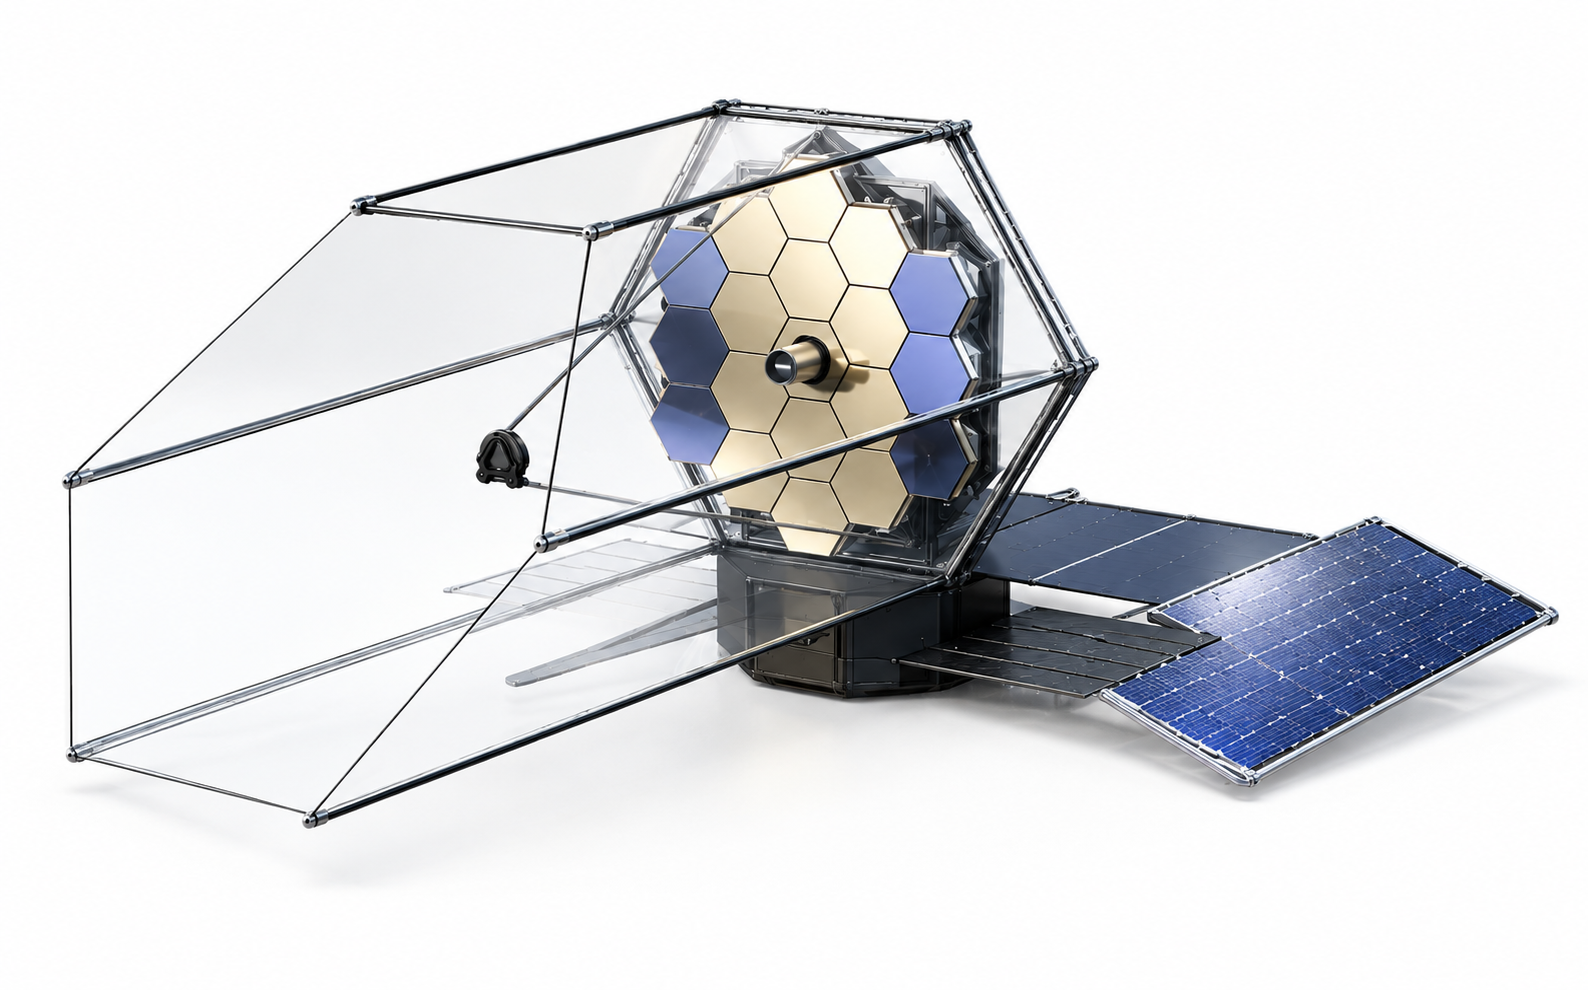
\includegraphics[width=\textwidth]{3.5ST_GPT.png}
  \vfill
  {\color{ink}\bfseries\normalsize \wpauthors\par}
  \vspace{3mm}
  {\color{muted}\small
    $^{1}$ Korea Institute for Advanced Study \textperiodcentered\
    $^{2}$ Korea Astronomy and Space Science Institute \\
    $^{3}$ University of Ulsan \textperiodcentered\
    $^{4}$ University of Science and Technology\\
    $^{5}$ Kyungpook National University \textperiodcentered\
    $^{6}$ Space Telescope Science Institute \textperiodcentered\
    $^{7}$ Pusan National University\\
    $^{8}$ Korea National University of Education \textperiodcentered\
    $^{9}$ Seoul National University \textperiodcentered\
    $^{10}$ Yonsei University\par}
  \vspace{5mm}
  {\color{Blue3}\bfseries\Large 2026}
  \vspace{4mm}
  \end{titlepage}}

\newcommand{\MakeColophon}{%
  \clearpage
  \thispagestyle{empty}\sffamily
  \null\vfill
  \noindent{\color{muted}\footnotesize
    {\color{ink}\bfseries 3.5-meter Segmented-Mirror Robotic Space Telescope}\\
    Mission White Paper: \wpvolumelabel. \wpvolumetitle\\[5mm]
    {\color{rose}\bfseries Release date September 1, 2026\\[5mm]}
    \textcopyright\ 2026 Korea Astronomy and Space Science Institute and the
    authors. All rights reserved.\\[2mm]
    Prepared by the mission study team at the Korea Astronomy and Space Science
    Institute, University of Ulsan, University of Science and Technology, the
    Space Telescope Science Institute, the Korea Institute for Advanced Study,
    Pusan National University, Korea National University of Education, Seoul
    National University, Kyungpook National University, and Yonsei University.\\[5mm]
    {\color{ink}\bfseries Suggested citation:} Kim, J., Kang, Y.-W., Lee, S.-H.,
    et al.\ (2026), \textit{3.5-meter Segmented-Mirror Robotic Space Telescope:
    Mission White Paper, \wpvolumelabel. \wpvolumetitle}.\\[2mm]
    {\color{ink}\bfseries Corresponding author:} Sang Hyun Lee
    \textperiodcentered\ \texttt{shlee@kasi.re.kr}.\par}
  \vspace{8mm}
  \clearpage}

\newcommand{\MakeBackCover}{%
  \clearpage
  \ifodd\value{page} \hbox{}\thispagestyle{empty}\newpage \fi
  \thispagestyle{empty}\null
  \clearpage
  \thispagestyle{empty}\sffamily\centering
  \null\vspace*{\stretch{1}}
  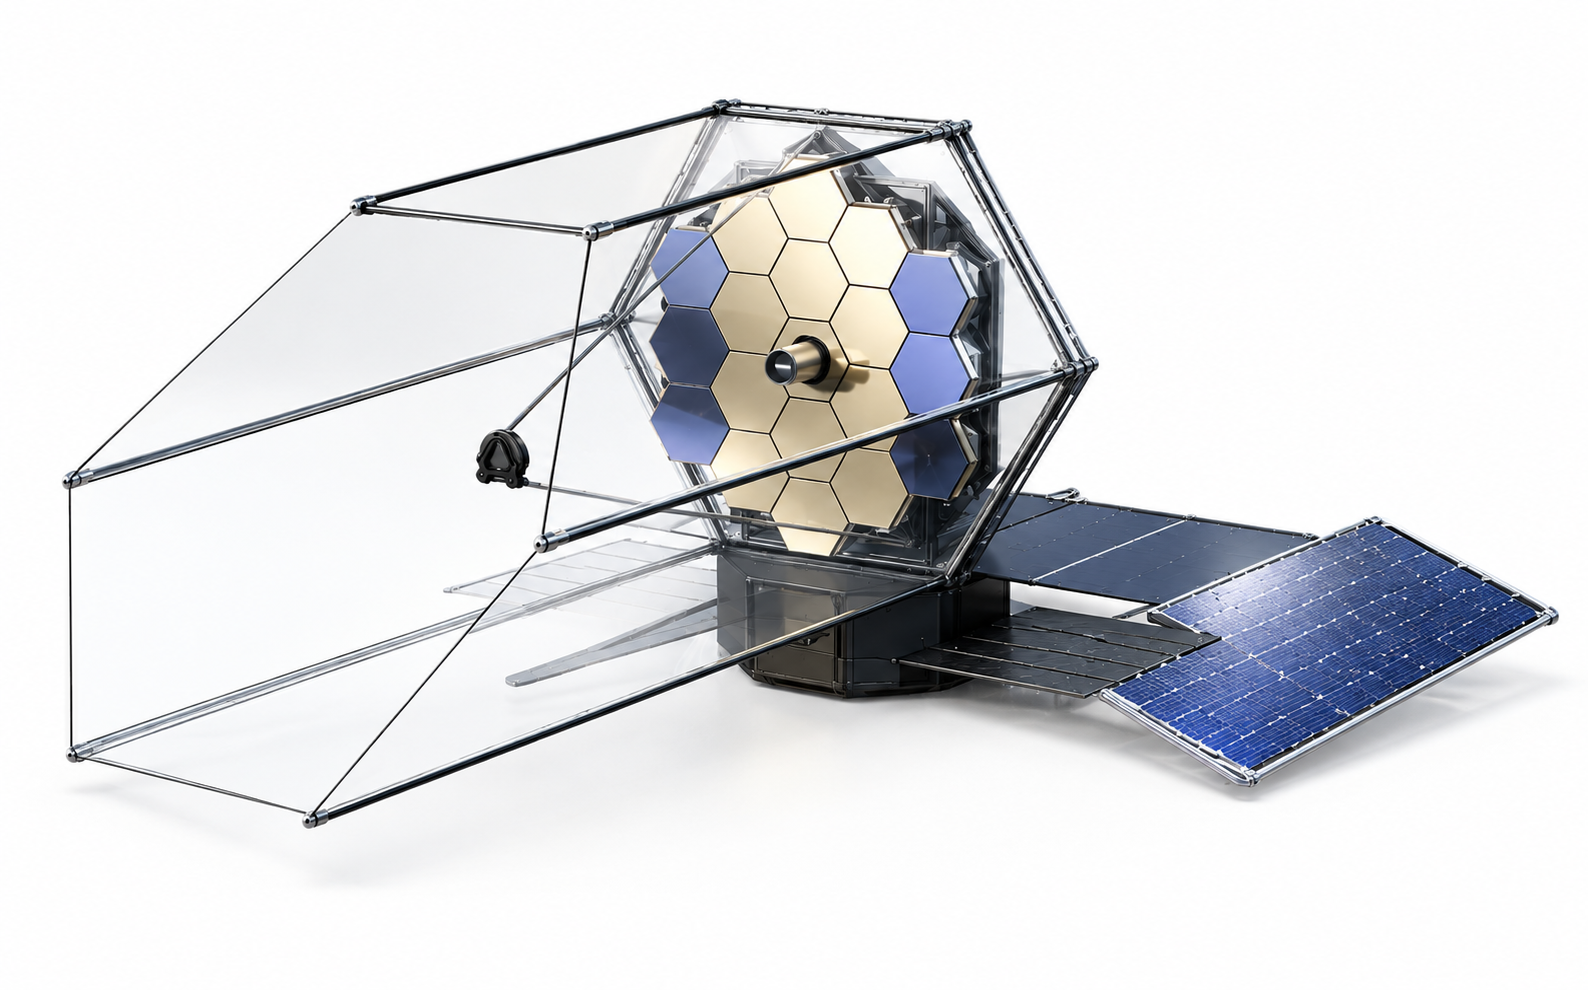
\includegraphics[width=\textwidth]{3.5ST_GPT.png}
  \vspace*{\stretch{2.2}}
  \noindent\colorbox{Blue3}{\parbox[t]{\dimexpr\textwidth-2\fboxsep\relax}{%
    \vspace{3mm}\centering
    {\color{white}\bfseries\Large 3.5-meter Segmented-Mirror Robotic Space Telescope}\\[1.5mm]
    {\color{white!88}\normalsize Mission White Paper: \wpvolumelabel. \wpvolumetitle}%
    \vspace{3mm}}}
  \vspace{3mm}
  \clearpage}
